\documentclass{fancyslides} 
\usepackage[utf8]{inputenc}
\usepackage{times}
\usepackage{listings}
\usepackage{hyperref}


%%% Beamer settings (do not change)
\usetheme{default} 
\setbeamertemplate{navigation symbols}{} %no navigation symbols
\setbeamercolor{structure}{fg=\yourowntexcol} 
\setbeamercolor{normal text}{fg=\yourowntexcol} 



%%%%%%%%%%%%%%%%%%%%%%%%%
%%% CUSTOMISATIONS %%%%%%
%%%%%%%%%%%%%%%%%%%%%%%%%

% THE FOLLOWING COLOURS ARE PREDEFINED IN THE CLASS
%bi -- WHITE
%cz -- BLACK
%sz -- GRAY
%nieb -- BLUE
%ziel -- GREEN
%pom -- ORANGE
%% YOU CAN DEFINE YOUR OWN COLOUR TO USE HERE. SEE MAN.PDF


%%%% SLIDE ELEMENTS
\newcommand{\structureopacity}{0.75} %opacity for the structure elements (boxes and dots)
\newcommand{\strcolor}{nieb} %elements colour (predefined nieb; pom; ziel)

%%%% TEXT COLOUR
\newcommand{\yourowntexcol}{bi}
\newcommand{\stext}[1]{{\color{black}#1}}
\newcommand{\ctext}[1]{{\ttfamily#1}}
\newcommand{\B}{\color{black}}
\newcommand{\tilda}{\raise.17ex\hbox{$\scriptstyle\sim$}}



%%%%%%%%%%%%%%%%%%%%%%%%%
%%% TITLE SLIDE DATA %%%%
%%%%%%%%%%%%%%%%%%%%%%%%%
\newcommand{\titlephrase}{Open~Geometry~Processing}
\newcommand{\name}{Alexandre Kaspar}
\newcommand{\affil}{EPFL / MIT}
\newcommand{\email}{akaspar@mit.edu}

\begin{document}

%\fontencoding{T1}
%\fontfamily{serif}
%\fontseries{m}
%\fontshape{it}
%\fontsize{12}{15}
%\selectfont

\lstset{
	language=C++,
    basicstyle=\color{black}\ttfamily,
    keywordstyle=\color{blue},
    identifierstyle=\color{gray!50!black},
    stringstyle=\color{green!50!black},
    commentstyle=\color{gray}\ttfamily\textit,
    morecomment=[l][\color{magenta}]{\#},
    numbers=left,
    numberstyle=\ttfamily,
    numbersep=10pt,
    xleftmargin=1cm
}

\setbeamercolor{frametitle}{fg=gray}

\startingslide %this generates titlepage from the data above

%%%%%%%%%%%%%%%%%%%%%%%%%
%%% SLIDES %%%%%%%%%%%%%%
%%%%%%%%%%%%%%%%%%%%%%%%%

%
%%%%%%%%%%%%%%%%%%%%%%%%%%%%%%%%%%%%%%%%%%%%%%%%%%%%%%%%%%%%%%%%%%%%%%%%%%%%%
%%%%% Introduction %%%%%%%%%%%%%%%%%%%%%%%%%%%%%%%%%%%%%%%%%%%%%%%%%%%%%%%%%%
%%%%%%%%%%%%%%%%%%%%%%%%%%%%%%%%%%%%%%%%%%%%%%%%%%%%%%%%%%%%%%%%%%%%%%%%%%%%%

%
% Content:
% 1. OpenMesh
% 2. Open Geometry Processing
% 3. Polygonal Meshes
%

%%%%%%%%%%%%%%%%%%%%%%%%%%%%%%%%%%%%%%%%%%%%%%%%%%%%%%%%%%%%%%%%%%%%%%%%%%%%%
\fbckg{backgrounds/3dparis2}
\begin{frame}
\pointedsl{OpenMesh}
\end{frame}

\setbeamercolor{frametitle}{fg=white}

\begin{frame}
\frametitle{OpenMesh}
\itemized{
	\item C++ library to work with polygonal meshes
	\item Half-edge data structure
	\item Efficient representation and manipulation
	\item Developed at the \href{http://www.graphics.rwth-aachen.de/}{Computer Graphics Group, RWTH Aachen}
	\item Led by Prof. Leif Kobbelt
}
\end{frame}

% based on http://www.openmesh.org/media/Documentations/OpenMesh-Doc-Latest/a00012.html
% more at http://opengp.github.io/tutorial.html

%%%%%%%%%%%%%%%%%%%%%%%%%%%%%%%%%%%%%%%%%%%%%%%%%%%%%%%%%%%%%%%%%%%%%%%%%%%%%
\setbeamercolor{frametitle}{fg=black}
\fbckg{backgrounds/3dparis-gray-edges}
\begin{frame}
\frametitle{OpenGP}
\framedsl{
	Open Geometry Processing?
}
\end{frame}

\begin{frame}
\frametitle{OpenGP}
\itemized{
	\item C++ library similar to OpenMesh
	\item Lightweight, simpler to use
	\item Developed at the \href{http://graphics.uni-bielefeld.de/}{Bielefeld Graphics \& Geometry Group}
	\item Led by Prof. Mario Botsch
}
\end{frame}

%%%%%%%%%%%%%%%%%%%%%%%%%%%%%%%%%%%%%%%%%%%%%%%%%%%%%%%%%%%%%%%%%%%%%%%%%%%%%
\fbckg{backgrounds/platonic}
\begin{frame}
\framedsl{
	Polygonal Meshes
}
\end{frame}

\begin{frame}
\frametitle{Polygons}
\itemized{
	\item Work with any $N$-gone faces
	\item Here focus on triangles
	\item Any polygon can be \emph{triangulated}
}
\end{frame}
%
%%%%%%%%%%%%%%%%%%%%%%%%%%%%%%%%%%%%%%%%%%%%%%%%%%%%%%%%%%%%%%%%%%%%%%%%%%%%%
%%%%% Traversing a mesh %%%%%%%%%%%%%%%%%%%%%%%%%%%%%%%%%%%%%%%%%%%%%%%%%%%%%
%%%%%%%%%%%%%%%%%%%%%%%%%%%%%%%%%%%%%%%%%%%%%%%%%%%%%%%%%%%%%%%%%%%%%%%%%%%%%
\fbckg{backgrounds/blank2}
\setbeamercolor{frametitle}{fg=gray}
\begin{frame}
\pointedsl{
	Using OpenGP
}
\end{frame}


%%%%%%%%%%%%%%%%%%%%%%%%%%%%%%%%%%%%%%%%%%%%%%%%%%%%%%%%%%%%%%%%%%%%%%%%%%%%%
\begin{frame}[fragile]
\frametitle{IO code}
\begin{lstlisting}
 // create empty mesh
Surface_mesh mesh;

// load .obj / .stl / .off
mesh.read("myfile.obj");

// process the mesh
// ...

// write the mesh to a file
mesh.write("myfile_processed.obj");
\end{lstlisting}
\end{frame}

\begin{frame}
\frametitle{Processing}
\misc{
	Reading and writing meshes is easy.
	
	Processing them is also easy. We will cover
	\begin{enumerate}
		\item Methods to \textbf{access connected elements}\\(i.e. edges, faces, vertices and their neighborhood)
		\item Ways to \textbf{traverse a mesh} (all faces, all boundary edges, all vertices around one vertex, etc.)
		\item How to \textbf{store data} on the mesh elements
		\item How to change the \textbf{topology} (add, delete elements)
	\end{enumerate}
}
\end{frame}
%
%%%%%%%%%%%%%%%%%%%%%%%%%%%%%%%%%%%%%%%%%%%%%%%%%%%%%%%%%%%%%%%%%%%%%%%%%%%%%
%%%%% Half-edge Data Structure %%%%%%%%%%%%%%%%%%%%%%%%%%%%%%%%%%%%%%%%%%%%%%
%%%%%%%%%%%%%%%%%%%%%%%%%%%%%%%%%%%%%%%%%%%%%%%%%%%%%%%%%%%%%%%%%%%%%%%%%%%%%
\fbckg{backgrounds/blank2}
\setbeamercolor{frametitle}{fg=gray}
\begin{frame}
\pointedsl{
	Half-Edges
}
\end{frame}

%
% Content:
% 1. What is a half-edge?
% 2. How are elements connected?
% 3. How do I work with half-edges?
% 4. How do I work with vertices? faces? edges?

%%%%%%%%%%%%%%%%%%%%%%%%%%%%%%%%%%%%%%%%%%%%%%%%%%%%%%%%%%%%%%%%%%%%%%%%%%%%%
\begin{frame}
\frametitle{Half-edges}
\begin{center}
	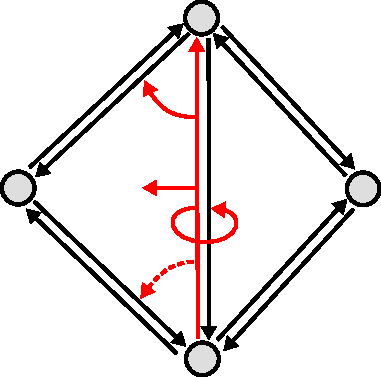
\includegraphics[width=0.42\textwidth]{figures/halfedge-connectivity}
\end{center}
\misc{
	Meshes are made of \emph{vertices}, \emph{edges} and \emph{faces}.
	
	Here, each edge is made of two \textbf{half-edges} (directed edges).
}
\end{frame}

%%%%%%%%%%%%%%%%%%%%%%%%%%%%%%%%%%%%%%%%%%%%%%%%%%%%%%%%%%%%%%%%%%%%%%%%%%%%%
\begin{frame}
\frametitle{Connectivity}
\begin{columns}[c]
  \begin{column}{0.4\textwidth}
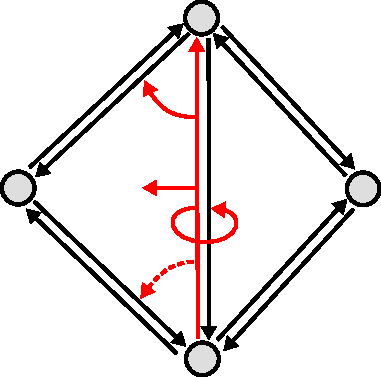
\includegraphics[width=\textwidth]{figures/halfedge-connectivity}
  \end{column}
  \begin{column}{0.6\textwidth}
\begin{itemize}
	\color{black}
	\item[\color{black}\textbullet] Each \textbf{vertex} is linked to an outgoing half-edge
	\item[\color{black}\textbullet] Each \textbf{face} is linked to an incident half-edge
	\item[\color{black}\textbullet] Each \textbf{half-edge} has \begin{itemize}
		\color{black}
		\item[\color{black}\textbullet] A next and previous half-edge
		\item[\color{black}\textbullet] A target vertex it points to
		\item[\color{black}\textbullet] An incident face
		\item[\color{black}\textbullet] An opposite half-edge\\(on the same edge)
	\end{itemize}
	\item[\color{black}\textbullet] Each \textbf{edge} has two corresponding half-edges
\end{itemize}
  \end{column}
\end{columns}
\end{frame}

%%%%%%%%%%%%%%%%%%%%%%%%%%%%%%%%%%%%%%%%%%%%%%%%%%%%%%%%%%%%%%%%%%%%%%%%%%%%%
\begin{frame}[fragile]
\frametitle{Half-edges code}
\begin{columns}[c]
  \begin{column}{0.4\textwidth}
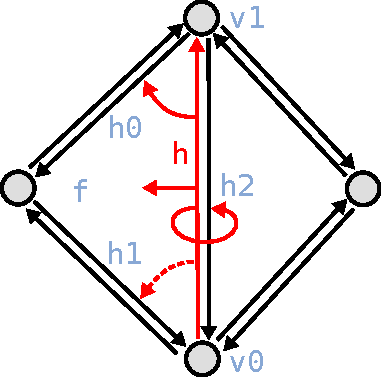
\includegraphics[width=\textwidth]{figures/halfedge-queries}
  \end{column}
  \begin{column}{0.6\textwidth}
  \lstset{ 
  	numbers=none, 
  	xleftmargin=0cm, 
  	xrightmargin=0cm
  }
\begin{lstlisting}
typedef Surface_mesh Mesh;

// the starting half-edge
Mesh::Halfedge h;
// the connected elements
Mesh::Halfedge h0, h1, h2;
Mesh::Face f;
Mesh::Vertex v0, v1;
\end{lstlisting}
  \end{column}
\end{columns}
\end{frame}

\begin{frame}[fragile]
\frametitle{Half-edges code}
\lstset{ numbers=none }
\begin{lstlisting}
// next half-edge
h0 = mesh.next_halfedge(h);
// previous half-edge
h1 = mesh.prev_halfedge(h);
// opposite half-edge
h2 = mesh.opposite_halfedge(h);
// incident face
f = mesh.face(h);
// vertex at source
v0 = mesh.from_vertex(h);
// vertex pointed by h
v1 = mesh.to_vertex(h);
\end{lstlisting}
\end{frame}

\begin{frame}[fragile]
\frametitle{Vertices, edges and faces}
\lstset{ numbers=none }
\begin{lstlisting}
// half-edge h of vertex v
h = mesh.halfedge(v);

// edge e of half-edge h
e = mesh.edge(h);
// half-edges h0,h1 from edge e
h0 = mesh.halfedge(e, 0);
h1 = mesh.halfedge(e, 1);

// half-edge h of face f
h = mesh.halfedge(f);

// checking if at the boundary
// same for h, e, f, v
bool b = mesh.is_boundary(h);
\end{lstlisting}
\end{frame}

%%%%%%%%%%%%%%%%%%%%%%%%%%%%%%%%%%%%%%%%%%%%%%%%%%%%%%%%%%%%%%%%%%%%%%%%%%%%%
\begin{frame}
\framedsl{
	Typedef!?
}
\end{frame}

\begin{frame}[fragile]
\misc{
	It creates a new name for a given type.
	
	Useful, especially when types are getting long and complex as
	it will be the case through these slides.
}
\lstset{ numbers=none }
\begin{lstlisting}
typedef my_long_complex_type new_type;

my_long_complex_type a;
// now equivalent to
new_type a;
\end{lstlisting}
\end{frame}

%%%%%%%%%%%%%%%%%%%%%%%%%%%%%%%%%%%%%%%%%%%%%%%%%%%%%%%%%%%%%%%%%%%%%%%%%%%%%
%%%%% Traversing a mesh %%%%%%%%%%%%%%%%%%%%%%%%%%%%%%%%%%%%%%%%%%%%%%%%%%%%%
%%%%%%%%%%%%%%%%%%%%%%%%%%%%%%%%%%%%%%%%%%%%%%%%%%%%%%%%%%%%%%%%%%%%%%%%%%%%%
\begin{frame}
\pointedsl{
	Exploration
}
\end{frame}

%
% Content:
% 1. Variables (declaration, assignment, operations)
% 2. Types (list: char, short, int, float, double, bool, void; typedef)
% 3. Expressions (unary, binary, arithmetic, comparator, bitwise)
% 4. Conditions (if, else if, else)
% 5. Loops (for, while, do while)
% 6. Arrays
% 7. Functions (declaration, definition, signature /!\ types -> diff fun)

%%%%%%%%%%%%%%%%%%%%%%%%%%%%%%%%%%%%%%%%%%%%%%%%%%%%%%%%%%%%%%%%%%%%%%%%%%%%%
\begin{frame}
\frametitle{Half-edges}
\begin{center}
	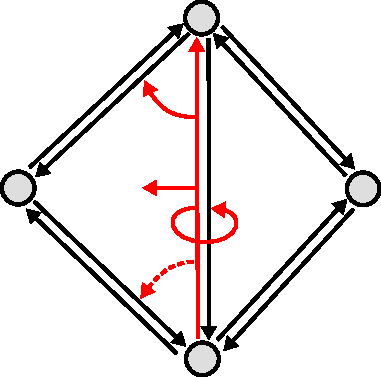
\includegraphics[width=0.5\textwidth]{figures/halfedge-connectivity}
\end{center}
\misc{
	Meshes are made of \emph{vertices}, \emph{edges} and \emph{faces}.
	
	Here, each edge is made of two half-edges (directed edges).
}
\end{frame}

\begin{frame}
\frametitle{Half-edges connectivity}
\begin{columns}[c]
  \begin{column}{0.4\textwidth}
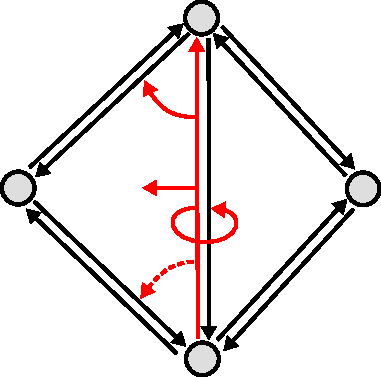
\includegraphics[width=\textwidth]{figures/halfedge-connectivity}
  \end{column}
  \begin{column}{0.6\textwidth}
\begin{itemize}
	\color{black}
	\item[\color{black}\textbullet] Each \textbf{vertex} is linked to an outgoing half-edge
	\item[\color{black}\textbullet] Each \textbf{face} is linked to an incident half-edge
	\item[\color{black}\textbullet] Each \textbf{half-edge} has \begin{itemize}
		\color{black}
		\item[\color{black}\textbullet] A next and previous half-edge
		\item[\color{black}\textbullet] A target vertex it points to
		\item[\color{black}\textbullet] An incident face
		\item[\color{black}\textbullet] An opposite half-edge\\(on the same edge)
	\end{itemize}
\end{itemize}
  \end{column}
\end{columns}
\end{frame}

\begin{frame}[fragile]
\frametitle{Half-edges code}
\begin{columns}[c]
  \begin{column}{0.4\textwidth}
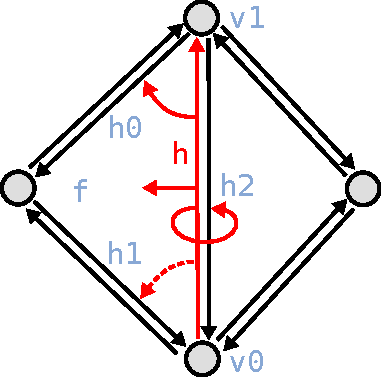
\includegraphics[width=\textwidth]{figures/halfedge-queries}
  \end{column}
  \begin{column}{0.6\textwidth}
  \lstset{ 
  	numbers=none, 
  	xleftmargin=0cm, 
  	xrightmargin=0cm
  }
\begin{lstlisting}
using Surface_mesh::Halfedge;
using Surface_mesh::Face;
using Surface_mesh::Vertex;

// the starting half-edge
Halfedge h;
// the connected elements
Halfedge h0, h1, h2;
Face f;
Vertex v0, v1;
\end{lstlisting}
  \end{column}
\end{columns}
\end{frame}

\begin{frame}[fragile]
\frametitle{Half-edges code}
\begin{lstlisting}
// next half-edge
h0 = mesh.next_halfedge_handle(h);
// previous half-edge
h1 = mesh.prev_halfedge_handle(h);
// opposite half-edge
h2 = mesh.opposite_halfedge_handle(h);
// incident face
f = mesh.face_handle(h);
// vertex at source
v0 = mesh.from_vertex_handle(h);
// vertex pointed by h
v1 = mesh.to_vertex_handle(h);
\end{lstlisting}
\end{frame}


%%%%%%%%%%%%%%%%%%%%%%%%%%%%%%%%%%%%%%%%%%%%%%%%%%%%%%%%%%%%%%%%%%%%%%%%%%%%%
%%%%% Storing data on the mesh %%%%%%%%%%%%%%%%%%%%%%%%%%%%%%%%%%%%%%%%%%%%%%
%%%%%%%%%%%%%%%%%%%%%%%%%%%%%%%%%%%%%%%%%%%%%%%%%%%%%%%%%%%%%%%%%%%%%%%%%%%%%
\fbckg{backgrounds/blank2}
\setbeamercolor{frametitle}{fg=gray}
\begin{frame}
\pointedsl{
	Properties
}
\end{frame}

%%%%%%%%%%%%%%%%%%%%%%%%%%%%%%%%%%%%%%%%%%%%%%%%%%%%%%%%%%%%%%%%%%%%%%%%%%%%%
\begin{frame}
\frametitle{Properties}
\misc{
	\textbf{Properties} of any kind (use of template) can be associated to
	\emph{vertices}, \emph{half-edges}, \emph{edges} or \emph{faces}.
	
	\begin{enumerate}
		\item How do we create them?
		\item How do we access them?
	\end{enumerate}
}
\end{frame}

\begin{frame}[fragile]
\frametitle{Property code}
\lstset{ numbers=none, xleftmargin=0cm }
\begin{lstlisting}
typedef Surface_mesh Mesh;

// storing Color data on each vertex
Mesh::Vertex_property<Color> colors;
colors = mesh.vertex_property<Color>("v:color");

// access property for vertex v
Mesh::Vertex v;
Color c = colors[v]; // get property
colors[v] = Color(0, 0, 0); // set black

// default position property
Mesh::Vertex_property<Point> points;
points = mesh.vertex_property<Point>("v:point");
\end{lstlisting}
\end{frame}

\begin{frame}[fragile]
\frametitle{Property code}
\begin{lstlisting}
// for element Xxx, storing type T
Mesh::Xxx_property<T> prop;
prop = mesh.xxx_property<T>(name);
// access with x of type Xxx
T t = prop[x];
\end{lstlisting}
\misc{
	where \ctext{Xxx} is one from 
	\ctext{Vertex}, \ctext{Face}, \ctext{Edge} or \ctext{Halfedge}.
	
	\phantom{x}
	
	The storage type \ctext{T} can be any common type (color, location, integer, float, etc.).
}
\end{frame}

\begin{frame}[fragile]
\frametitle{Normal properties}
\misc{
	Normals (of type \ctext{Normal}) can be computed automatically and are available in two flavors: per-vertex (property \ctext{"v:normal"}) of per-face (property \ctext{"f:normal"}).
}
\lstset{ numbers=none, xleftmargin=0cm}
\begin{lstlisting}
// compute normals
mesh.update_vertex_normals();

// access normals
Mesh::Vertex_property<Normal> nrs;
nrs = mesh.vertex_property<Normal>("v:normal");
Normal n = nrs[v];
\end{lstlisting}
\end{frame}


%%%%%%%%%%%%%%%%%%%%%%%%%
%%% ENDING %%%%%%%%%%%%%%
%%%%%%%%%%%%%%%%%%%%%%%%%

\fbckg{backgrounds/blank2}
\begin{frame}
  \thankyou   %%%% ending slide with thank you notice
\end{frame}

\begin{frame}
\sources{

\includegraphics[height=1em]{figures/bunny-logo} \ \href{http://www.graphics.rwth-aachen.de/}{Graphics at RWTH Aachen}\\

\includegraphics[height=1em]{figures/bunny-logo} \ OpenMesh: \url{http://www.openmesh.org}\\

\includegraphics[height=1em]{figures/bunny-logo} \ OpenGP: \url{http://opengp.github.io	}
}
\end{frame}


\end{document}